\documentclass[]{beamer}
\usepackage[parfill]{parskip}    % Activate to begin paragraphs with an empty line rather than an indent
\usepackage{graphicx}
\usepackage{amssymb}
\usepackage{epstopdf}
\usepackage{natbib}
\usepackage{setspace}
\usepackage{hyperref}
\usepackage{svninfo}
\svnInfo $Id: presentation.tex 646 2009-07-08 12:35:02Z baart_f $
\usepackage{listings}
\def\newblock{}

\definecolor{citecolor}{rgb}{0.0,0.6,0.6}
\definecolor{filecolor}{rgb}{1.0,0.0,0.0}
\definecolor{linkcolor}{rgb}{0.8,0.8,1.0}
\definecolor{urlcolor}{rgb}{0.29,0.28,0.74} % same color as Antibes middle bar

\hypersetup{colorlinks,%
            citecolor=citecolor,%
            filecolor=filecolor,%
            linkcolor=linkcolor,%
            urlcolor=urlcolor,%
            pdftex}

%\usetheme{Frankfurt
%\usetheme[secheader]{Madrid}
%\usetheme{Berkeley}
\usetheme{Berlin}
\usecolortheme{rose}

\setbeamercovered{transparent}


\setbeamertemplate{blocks}[rounded][shadow=true]


\title{OpenDAP configuration course}
\author{Fedor Baart}
\date{\today  (revision \svnInfoRevision)}       

\begin{document}

\frame{\titlepage}


\section[Outline]{}
\frame{\tableofcontents}

\section{Introduction}
\frame
{
  \frametitle{Time schedule}
  \begin{itemize}
  \item{13:00 - 13:30} Project overview
  \item{13:30 - 14:00} System architecture
  \item{14:00 - 14:45} System setup excercise
  \item{14:45 - 15:00} Coffee break
  \item{15:00 - 15:30} NetCDF introduction
  \item{15:30 - 16:15} Configuration excercise
  \item{16:15 - 17:00} Tweaking
  \end{itemize}


}
\section{Overview}
\frame
{
  \frametitle{Projects using OpenDAP}
  \begin{itemize}
  \item MICORE
  \item BwN
  \item Matroos
  \end{itemize}
}
\frame
{
  \frametitle{MICORE}
  \begin{figure}[htbp]
   \centering
   \includegraphics[width=10cm]{/Users/fedorbaart/Documents/checkouts/baart_f/documents/pictures/micore/sites.png} % requires the graphicx package
   \caption{Overview of micore sites}
   \label{fig:processes}
\end{figure}
}

\frame
{
  \frametitle{MICORE}
  June 2008 - June 2011
  \begin{itemize}
  \item Historical storms (UALG, PT)
  \item Data standards (TUD, NL)
  \item Site monitoring (BRGM, FR)
  \item Modelling (Deltares, NL)
  \item Warning system (IMDC, BE)
  \item Dissemination (SGSS, IT)
  \item Project management (CFR Ufe, IT)
  \end{itemize}
}

\frame
{
  \frametitle{Building with Nature}
  \note{Find a better description, this one is from the website}
  Building with Nature is an innovative, long-term  
  research programme aimed at developing new design 
  concepts for the layout and sustainable exploitation of 
  river, coastal and delta areas. Its special feature is the 
  synergy and cooperation that will allow natural ecosystems and human intervention to reinforce each other. 
  Ecology and technology are involved at all phases of a 
  project: design, assessment, selection, construction and 
  management. The primary goal is ecologically, technically and socially sustainable development. 
}

\frame
{
  \frametitle{Building with Nature Partners}
  \note{this list doesn't fit}
  \begin{itemize}
  \item Boskalis
  \item Van Oord
  \item IHC Merwede
  \item Deltares
  \item IMARES 
  \item SHELL
  \item Witteveen + Bos
  \item DHV
  \item Royal Haskoning
  \item Technical University Delft
  \item Wageningen University
  \item University of Twente
  \item Astron
  \item RWS-Bouwdienst
  \item NIOZ
  \item NIOO-CEME
  \item VBKO
  \item City of Dordrecht
\end{itemize}
}

\frame
{
  \frametitle{Matroos}
  \note{some pictures would be good here}
  MATROOS stands for Multifunctional Access Tool foR Operational Oceandata Services. MATROOS gives you easily access using your internet browser to all recent and historical model and monitoring data relevant to the storm surge forecasts. MATROOS offers also the facility of an international near-real time multi-model forecast analysis: water level forecasting data and weather forecasting data from the NOOS partners around the North Sea can be intercompared.
}

\section{Architecture}
\frame
{
  \frametitle{Process}

  \begin{figure}[htbp]
   \centering
   \includegraphics[type=png,width=10cm,read=.png,ext=.png]{/Users/fedorbaart/Documents/checkouts/baart_f/documents/presentations/lunch/presentation/micore.005} % requires the graphicx package
   \caption{Steps in data processing}
   \label{fig:processes}
\end{figure}
}

\frame
{
  \frametitle{Extract}

  \begin{figure}[htbp]
   \centering
   \includegraphics[type=png,width=10cm,read=.png,ext=.png]{/Users/fedorbaart/Documents/checkouts/baart_f/documents/presentations/lunch/presentation/micore.006} % requires the graphicx package
   \caption{Extraction process}
   \label{fig:processes}
\end{figure}
}


\frame
{
  \frametitle{Transform}

  \begin{figure}[htbp]
   \centering
   \includegraphics[type=png,width=10cm,read=.png,ext=.png]{/Users/fedorbaart/Documents/checkouts/baart_f/documents/presentations/lunch/presentation/micore.007} % requires the graphicx package
   \caption{Import aspects of transformation}
   \label{fig:processes}
\end{figure}
}


\frame
{
  \frametitle{Load}

  \begin{figure}[htbp]
   \centering
   \includegraphics[type=png,width=10cm,read=.png,ext=.png]{/Users/fedorbaart/Documents/checkouts/baart_f/documents/presentations/lunch/presentation/micore.008} % requires the graphicx package
   \caption{Provide}
   \label{fig:processes}
\end{figure}
}

\frame
{
  \frametitle{Services}

  \begin{figure}[htbp]
   \centering
   \includegraphics[type=png,width=10cm,read=.png,ext=.png]{/Users/fedorbaart/Documents/checkouts/baart_f/documents/presentations/lunch/presentation/micore.009} % requires the graphicx package
   \caption{Service layer}
   \label{fig:processes}
\end{figure}
}

\frame
{
  \frametitle{Provide}

  \begin{figure}[htbp]
   \centering
   \includegraphics[type=png,width=10cm,read=.png,ext=.png]{/Users/fedorbaart/Documents/checkouts/baart_f/documents/presentations/lunch/presentation/micore.010} % requires the graphicx package
   \caption{Provide}
   \label{fig:processes}
\end{figure}
}


\section{Components}
\frame{
  \frametitle{Extract}
  \begin{block}{Software}
  \begin{itemize}
  \item \emph{Subversion} provides version history, logging, changesets and filesystem storage for the raw data. The \href{http://subversion.tigris.org/}{subversion server} comes with the command line client.
  \item \emph{Apache} provides \href{http://httpd.apache.org/docs/2.2/howto/auth.html}{authentication and authorization}. Provides \href{http://httpd.apache.org/docs/2.2/mod/mod_dav.html}{webdav} for drive mapping. 
  \end{itemize}
  \end{block}
  \begin{block}{Hardware}
  \begin{itemize}
  \item A \emph{fileserver} is needed to store subversion repository. At Deltares we use \href{http://www.drbd.org/}{drbd} for high availability.
  \item \emph{Backup} is needed to backup the repository.
  \end{itemize}
  \end{block}
}

\frame{
  \frametitle{Transform}
    \begin{block}{Software}
  \begin{itemize}
      \item \emph{NetCDF} itself should be installed as a \href{http://www.unidata.ucar.edu/software/netcdf/docs/netcdf-install/}{library} (dll for windows). Extra tools like \href{http://nco.sourceforge.net/}{nco} and \href{http://www.mpimet.mpg.de/fileadmin/software/cdo/}{cdo} for altering and combining netCDF files and \href{http://www.gfdl.noaa.gov/~vb/grids/gridspec-tools.html}{gridspec-tools}. 
    \item \emph{Matlab\textsuperscript{\texttrademark}} is used for creating netCDF files from the raw data.  Extra libraries required are \href{http://mexcdf.sourceforge.net/}{mexnc} and \href{http://public.deltares.nl/display/OET/OpenEarth}{OpenEarthTools}. 
    \item \emph{Python} is also used for creating netCDF files. Extra libraries are \href{http://www.scipy.org/}{scipy} and \href{http://code.google.com/p/netcdf4-python/}{netcdf4-python}
      \item \emph{Inspire} guidelines are used to adhere to the ISO19115/119 standards. Use the \href{http://www.inspire-geoportal.eu/InspireEditor/}{editor} to fill in metadata.
  \end{itemize}
  \end{block}
  \begin{block}{Hardware}
    Just a computer which can do some calculations.
  \end{block}
}


\frame{
 \frametitle{Load}
    \begin{block}{Software}
  \begin{itemize}
    \item \emph{OpenDAP} server for giving access to generated netCDF files. We use \href{http://opendap.org/download/hyrax.html}{hyrax} and \href{http://www.unidata.ucar.edu/projects/THREDDS/}{thredds}. `
    \item \emph{Tomcat} runs java web applications. It is quite easy to \href{http://tomcat.apache.org/tomcat-6.0-doc/index.html}{setup}. 
    \item \emph{Apache} runs as a reverse proxy in front  of the tomcat, also again auth \& auth.
  \end{itemize}
  \end{block}
  \begin{block}{Hardware}
  \begin{itemize}
    \item \emph{Fileserver} should host the netcdf files. This one should probably be inside the \href{http://en.wikipedia.org/wiki/DMZ_\%28computing\%29}{DMZ}. Use \href{http://en.wikipedia.org/wiki/Secure_copy} to upload files. 
    \item \emph{Application server} should host the Tomcat application.  On the same machine as the fileserver for performance.
  \end{itemize}

  \end{block}
}

\frame{
 \frametitle{Provide}
    \begin{block}{Software}
  \begin{itemize}
    \item \emph{OpenEarthTools} contains a lot of matlab\textsuperscript{\texttrademark} tools to work with the datasets. 
    \item \emph{Open Source GUI} tools for displaying and browsing netCDF files and opendap servers. Examples are \href{http://www.epic.noaa.gov/java/ncBrowse/}{ncbrowse}, \href{http://www.unidata.ucar.edu/software/idv/}{IDV}, \href{http://www.unidata.ucar.edu/downloads/netcdf/netcdf-java-4/index.jsp}{netcdf-ui}.
    \item \emph{Geoserver} server for running OGC services. Also a Tomcat application.
  \end{itemize}
  \end{block}
  \begin{block}{Hardware}
  \begin{itemize}
    \item \emph{Application server} should host Tomcat application.  
  \end{itemize}

  \end{block}
}


\frame
{
  \frametitle{Hyrax}
  \note{create better figure explaining differences between hyrax,thredds dap, remove reference to sql data, check if tonnetje refers to database or storage}
  \begin{figure}[htbp]
   \centering
   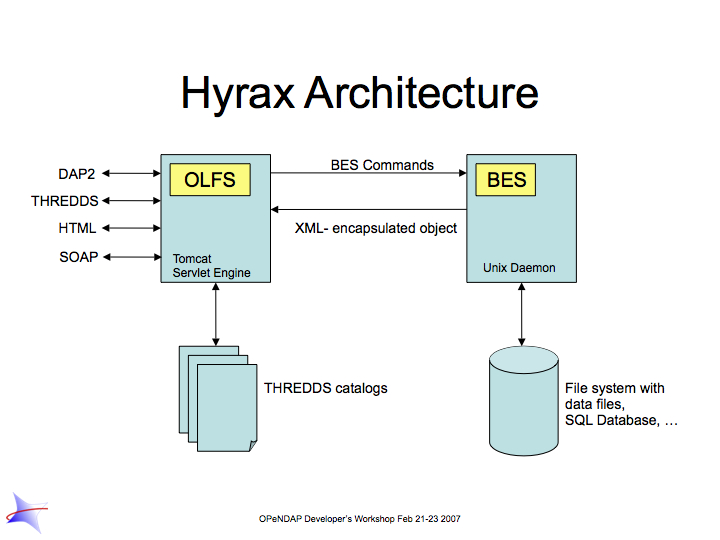
\includegraphics[width=10cm]{HyraxArchitecture.jpg} % requires the graphicx package
   \caption{Hyrax architecture}
   \label{fig:processes}
\end{figure}
}



\section{Hyrax}
\frame
{
  \frametitle{System setup excercise}
  \begin{itemize}
  \item[$\rightarrow$] \url{http://www.opendap.org}
  \item[$\rightarrow$] download
  \item[$\rightarrow$] hyrax
  \end{itemize}
}

\frame
{
  \frametitle{Downloading software}
  \begin{itemize}
  \item download OLFS web archive
  \item download all rpm's below Linux CentOS 5.2 (i386)
  \item download tomcat 6
  \end{itemize}
}

\begin{frame}[fragile]
  \frametitle{Extract rpms}
\begin{block}{Extract rpms}
  \lstset{language=bash}
  \begin{lstlisting}
    rpm2cpio filename.rpm | cpio -idmv
\end{lstlisting}
\end{block}
\end{frame}


\subsection{Backend server}
\begin{frame}[fragile]
  \frametitle{Copy \& Change script}
  

  \lstset{language=bash}
  \begin{block}{move to  your home directory}
  \begin{lstlisting}
    mv usr etc var ~
  \end{lstlisting}
  $\rightarrow$ Edit the besctl file to refer to $\sim$ instead of /usr/bin
  \end{block}


\end{frame}



\subsection{Backend configuration}

\begin{frame}[fragile]
  \frametitle{Edit the configuration so it refers to your home directory}
 \lstset{language=bash}
 \begin{block}{edit configuration}
  \begin{lstlisting}
    emacs -nw ~/etc/bes.conf
  \end{lstlisting}
  \end{block}

\end{frame}

\subsection{Run}
\begin{frame}[fragile]
  \frametitle{Run the backend server}
 \lstset{language=bash}
 \begin{block}{start bes}
  \begin{lstlisting}
    cd ~/usr/bin
    ./besctl start
  \end{lstlisting}
  \end{block}
  \begin{block}{Create the directory $\sim$/var/run}
  \begin{lstlisting}
    mkdir ~/var/run
    cd ~/usr/bin
    ./besctl start
  \end{lstlisting}
  \end{block}

\end{frame}

\section{Frontend}
\begin{frame}[fragile]
  \frametitle{Extract tomcat server}
  

  \lstset{language=bash}
  \begin{block}{Extract the java components of the server}
  \begin{lstlisting}
    tar -xzf apache-tomcat-6.tar.gz
    tar -xzf olfs-webapp.tgz
  \end{lstlisting}
  
  \end{block}


\end{frame}


\section{NetCDF}
\frame
{
  \frametitle{NetCDF Data Model}
  \begin{figure}[htbp]
   \centering
   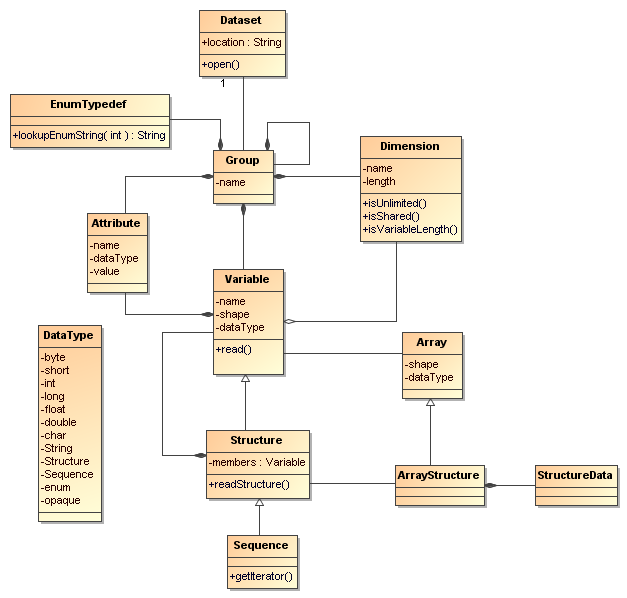
\includegraphics[width=10cm]{CDM-UML.png}
   \caption{Data model}
   \label{fig:processes}
\end{figure}

}


\section{Extra}
\frame
{
  \frametitle{Extra excercise}
  \begin{itemize}
    \item Setup thredds server (15min)
    \item Configure thredds server (45min)
    \item Security settings (30min)
    \item Look at url rewriting (30min)
    \item Caching (30min)
    \item Command line tools (30min)
  \end{itemize}

}


  \bibliographystyle{apalike}
  \bibliography{bibliography}

\end{document}  